{
\subsection{Объем тела вращения. Объем тела с известными площадями поперечных сечений. Объем эллипсоида.}
\subsection*{Теорема: Объем тела вращения}
\[
\text{Пусть } f \in C[a, b], \quad f \geq 0 \text{ на } [a, b].
\]
Объём \( V \) тела \( T \), полученного путём вращения подграфика \( y = f(x) \) вокруг оси \( OX \), равен:

\begin{figure}[h]
    \centering
    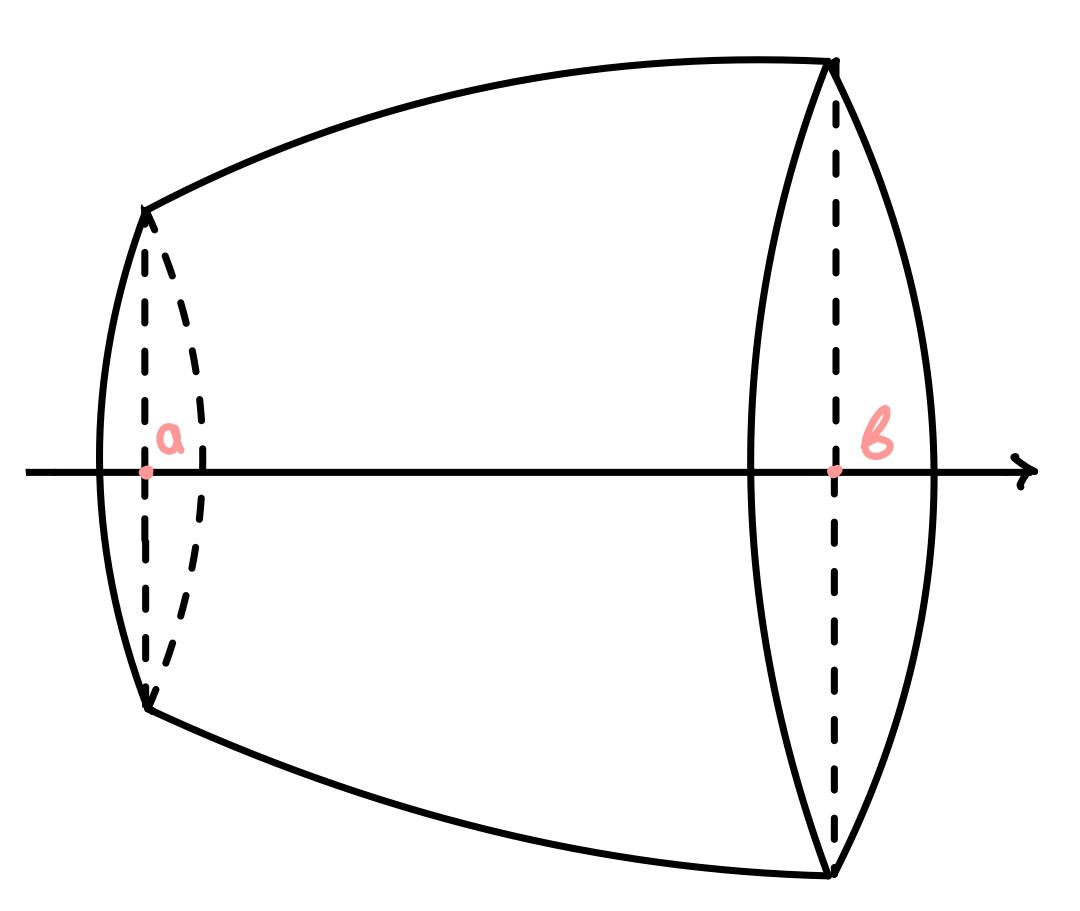
\includegraphics[width=0.4\linewidth]{source/image.png}
    \label{fig:rotation}
\end{figure}

\[
V = \pi \int_a^b f^2(x) \, dx.
\]

\subsection*{Объем тела с известными площадями поперечных сечений}
Рассмотрим тело \( T \), заключенное между плоскостями \(x = a, x = b\).

Пусть \(Q(x) \) - фигура, полученная при сечении тела плоскостью \(x = const,(x \in [a,b]) \)

Пусть \(Q(x) \) - фигура, полученная при сечении тела плоскостью \(\forall \, x \in [a,b] \) и функция \(S(x) = S(Q(x))\) непрерывна на \([a,b]\).

\begin{figure}[h]
    \centering
    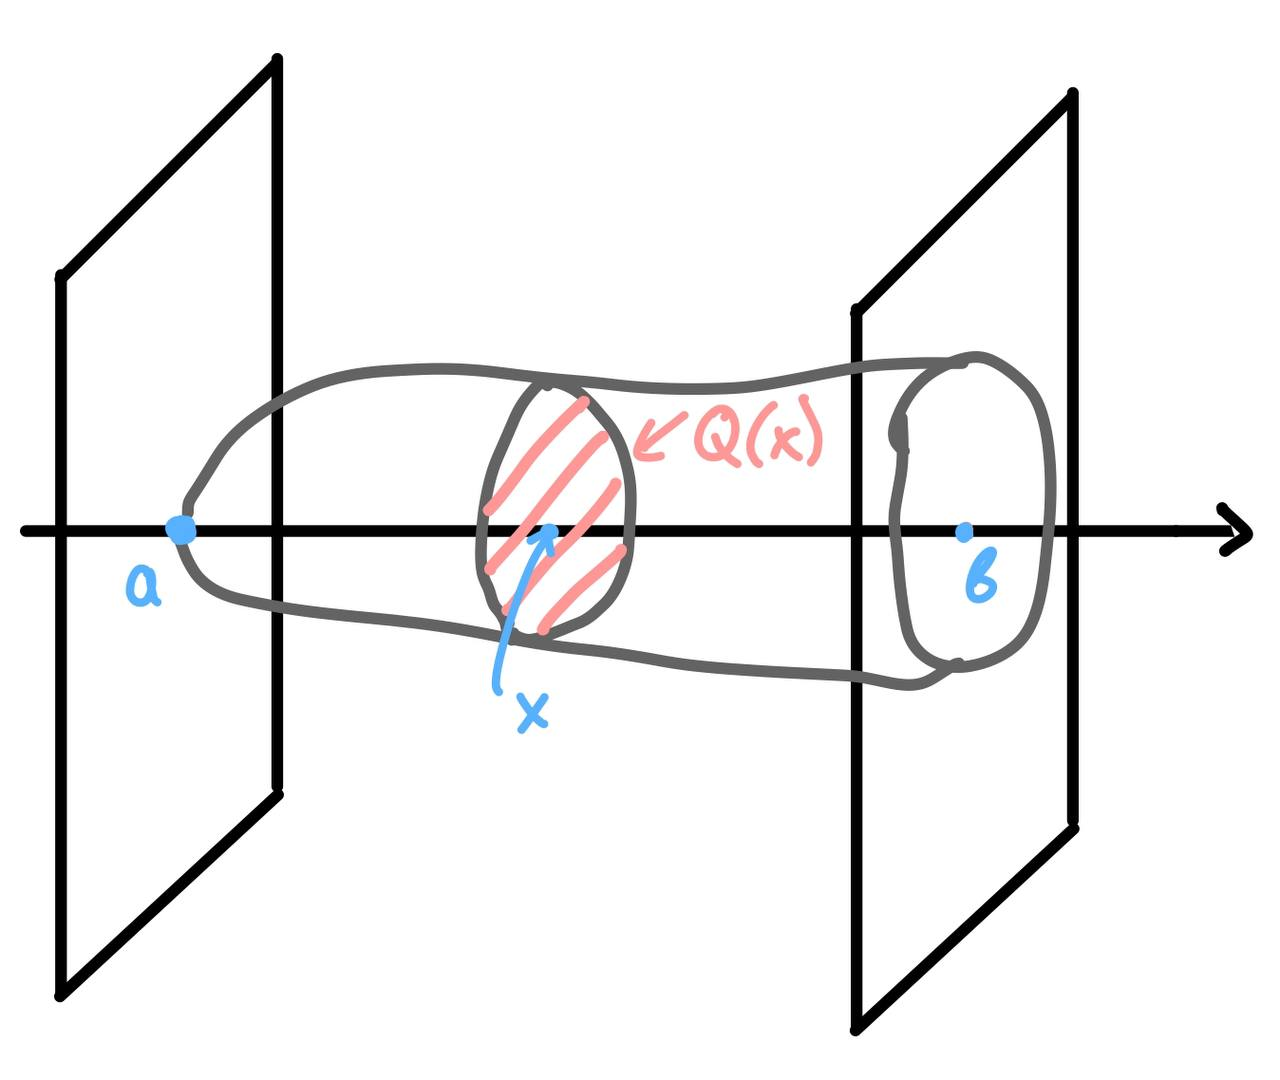
\includegraphics[width=0.4\linewidth]{source/2.png}
    \label{fig:enter-label}
\end{figure}
\[ \text{Тогда \,}V = \int_a^b{S(x) \, dx}\]
\newpage
\subsection*{Объем элипсоида}
\[
\frac{x^2}{a^2} + \frac{y^2}{b^2} + \frac{z^2}{c^2} = 1
\]

В сечении элипсоида пл-тью \( x = x_0\) имеем эллимсоида пл-тью
\[
\frac{y^2}{b^2} + \frac{z^2}{c^2} = 1 - \frac{x_0^2}{a^2} \iff \frac{y^2}{\left[ b \, \sqrt{1 - \frac{x_0^2}{a^2}}\right]^2} + \frac{z^2}{\left[ c  \, \sqrt{1 - \frac{x_0^2}{a^2}}\right]^2} = 1
\]
\[ \Rightarrow \text{площадь сечения } S(x_0) = \pi b_1 c_1 = \pi b c \left( 1- \frac{x_0^2}{a^2} \right)\]
\[ \Rightarrow V = \int_{-a}^{a}{S(x) \, dx} = \int_{-a}^{a}{\pi b c \left( 1- \frac{x_0^2}{a^2} \right)} \, dx \]  
\[= \pi b c \left[ (a - \frac{a^3}{3a^2}) - (-a + \frac{a^3}{3a^2}) \right] = \pi b c \left( 2a-\frac{2}{3} \right) = \frac{4}{3}\pi a b c\]
\subsection*{Следствие}
Обьем шара радиуса \( R \, (a=b=c=R)\), есть \(\frac{4}{3}\pi R^3\)
}